% This is a sample document using the University of Minnesota, Morris, Computer Science
% Senior Seminar modification of the ACM sig-alternate style. Much of this content is taken
% directly from the ACM sample document illustrating the use of the sig-alternate class. Certain
% parts that we never use have been removed to simplify the example, and a few additional
% components have been added.

% See https://github.com/UMM-CSci/Senior_seminar_templates for more info and to make
% suggestions and corrections.

\documentclass{sig-alternate}
\usepackage{color}

%%%% User-defined macros
\newcommand{\lam}{\lambda}
\newcommand{\mycomment}[1]{\textcolor{red}{#1}}
\newcommand{\vm}[0]{virtual machine}
%%%%% Uncomment the following line and comment out the previous one
%%%%% to remove all comments
%%%%% NOTE: comments still occupy a line even if invisible;
%%%%% Don't write them as a separate paragraph
%\newcommand{\mycomment}[1]{}

\begin{document}

% --- Author Metadata here ---
%%% REMEMBER TO CHANGE THE SEMESTER AND YEAR
\conferenceinfo{UMM CSci Senior Seminar Conference, April 2014}{Morris, MN}

\title{Programming Language Interoperability}

\numberofauthors{1}

\author{
% The command \alignauthor (no curly braces needed) should
% precede each author name, affiliation/snail-mail address and
% e-mail address. Additionally, tag each line of
% affiliation/address with \affaddr, and tag the
% e-mail address with \email.
\alignauthor
Todd Malone\\
	\affaddr{Division of Science and Mathematics}\\
	\affaddr{University of Minnesota, Morris}\\
	\affaddr{Morris, Minnesota, USA 56267}\\
	\email{malon153@morris.umn.edu}
}

\maketitle
\begin{abstract}
\mycomment{A discussion of systems and methods for the interop of programming languages}
\end{abstract}

\keywords{interoperability, language interoperability, programming languages, virtual machines, markup languages}

\section{Introduction}
Interoperability, colloquially shortened to interop, is the ability for two or more systems to work together. This definition is very broad, covering anything from groups of people to businesses or bureaucratic systems to pieces of hardware. This paper will discuss interoperability between programming languages. While this narrows the field quite a bit, programming language interop is still a very large topic.

For instance, all browsers perform some kind of interop. Information to be displayed on a web page is handled by HTML, and anything that along with PHP or Javascript, but if there is more computation to be done, or if a database needs to be consulted, these frontend languages will communicate with a server, often written in languages like Java or C.

Likewise, these servers may be written in several languages themselves. A blog hosting service, KidBlog, uses a backend written in both Java and Clojure \mycomment{for reasons}

The challenges that arise when dealing with interoperability can be many, and sometimes surprising. The tools and approaches used to counter these challenges are likewise many. In the interest of brevity, we will look at a small subset of these challenges, along with several tools used to deal with them.

In Section \ref{Interop} I'll explore why interoperability is desirable, what advantages it can confer, and where it can be useful. This will touch on differing language capabilities, ease of use, hardware independence, and implications for distributed computing.

Next, in Sections \ref{VM} and \ref{ML}, I'll describe two particular tools that are used to achieve interoperability, and defining relevant aspects of these settings. These tools will be virtual machines, paying particular attention to the Java Virtual Maching (JVM) and .NET's Common Language Runtime (CLR), and markup languages, with focus on two particular systems that make use of markup languages, Starlink and FML.

Section \ref{approaches} will detail particular challenges involved with interoperability and approaches to handling them. Following a general description of the approach, I will describe how each tool can be used to implement that approach, along with strengths and weaknesses of each setting.

Section \ref{performance} will look at a few of the performance implications of the tools discussed.


\section{Interoperability}\label{Interop}
Why is interoperability something anyone cares about? One of the primary reasons is that different languages simply perform better in certain circumstances. Early on in Java's life, for instance, it was intended to be the go-to language for the web. In practice now, however, it has been outpaced by languages like JavaScript or Flash, and is primarily used to run server architecture or programs on personal computers. \mycomment{citation from early java paper. Also, why did these replace Java? remove if can't find reason.}



Other languages are built to handle particular problems, while providing almost no support for others. Erlang, for instance, is one of the primary languages used in distributed computing. It was built around remote procedure calls (RPCs), and handles them simply and powerfully. However, manipulating strings in Erlang is very difficult, because Erlang was never intended to deal with strings. As a result, it has no library for string interaction, and treats them as arrays of characters. A system using Erlang for handling distributed communications which also needed to manipulate strings would have use for interop: another language could be used to handle the strings, while leaving the RPCs to Erlang.

Still others allow access in ways that are hidden in other languages. The memory access model in C, for instance, differs from many other high-level languages presently in use. C enables very fine-grained memory access and control, and places all of this control in the programmer's hands.


Apart from the capabilities of the languages involved, interoperability is often tied to hardware independence. The problems faced in achieving language independence and hardware independence are frequently similar, or have similar solutions. As noted above in the case of Java, designing for hardware independence allowed the JVM to act as a tool for language independence as well.

\begin{itemize}

	
	\item Peformance: lower-level languages, assembly, have direct access to hardware. This allows some things that more abstract languages, like Java, Ruby, Python, simply cannot do. One of these things is performance. Direct access to hardware allows programmers to make very fined-tuned adjustments that are program or intent specific - too specific for a compiler to reasonably translate them from a more abstract language. 
	Additionally, certain programs need hardware access to be useful. \mycomment{I could talk about device drivers like Nic suggested, but are there many others that need both hardware access and abstract structures?}
	\mycomment{does C offer hardware access? if not, why is it used for writing OS's?}
		
	\item Hardware independance and distributed computing: While interoperability doesn't require these, it can often enable them or result as a side effect of achieving either.
	
	Hardware independence frequently involves writing interpreters for a language that target different hardware systems. In the case of Java, this was done by translating Java into a lower-level language that was easier to write platform-specific runtimes for.
	\mycomment{I need a citation. Additionally, make sure this last bit is actually true}
	Although unintended, this intermediate language provided an opportunity for other languages to interoperate with Java.	
	
	Distributed computing often involves sending data in largely unformatted streams. Because formatting may be needed on the other side, formatting data also must be sent, which can be used by a any language or program that is able to parse the formatting information. I'll take a closer look at this in section \ref{metadata}.
\end{itemize}


\section{Virtual Machines}\label{VM}
\begin{figure}
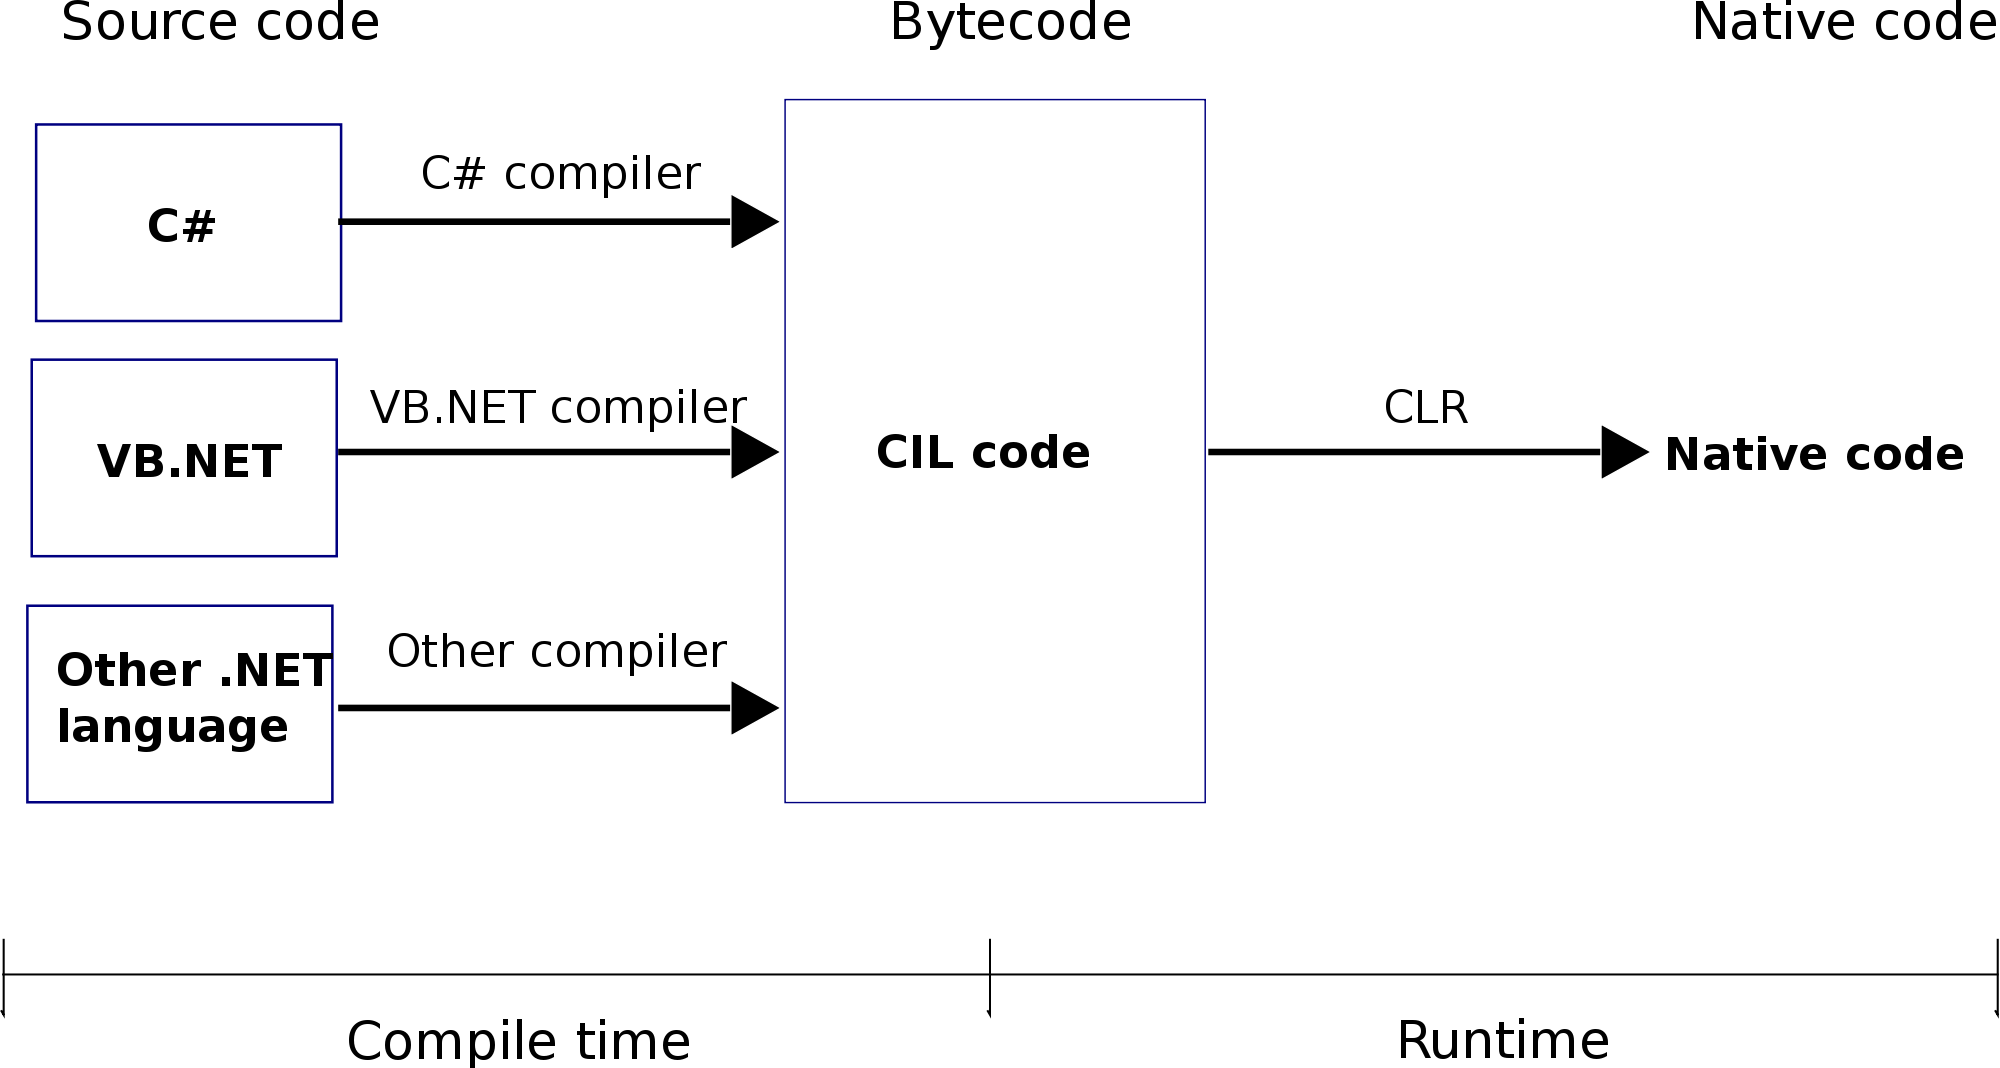
\psfig{file=CLR.png, width = 3in}
\caption{VM architecture: The CLR}
\end{figure}

The term virtual machine (VM) refers to software that models the operating system of a computer or the underlying physical hardware. Effectively, VMs are indistinguishable from the OS or hardware they are emulating, which allows them to run programs not runable by the native OS, or with restrictions not enforced by the native OS or hardware.
The focus of this paper will be on virtual machines that act as a runtime environment for a single process, sometimes called process VMs. These VMs in particular enforce restrictions on what system resources their hosted process has access too. Specifically, they typically provide restricted, VM managed memory spaces, ensuring that hosted processes can't access memory beyond what is allocated to it.\cite{wiki:VM} \mycomment{is this relevant?}

There are two major advantages to virtual machines. The first of these is a type safety mechanism. Virtual machines such as the Java Virtual Machine (JVM) and .NET's Common Language Runtime (CLR) have a base set of types (in the CLR, this is actually called the Common Type System, or CTS. It is implicit and unnamed in the JVM). The VMs can use these type systems to ensure the correctness of participating languages and gives languages a common ground for their type information.

The second advantage lies in the VM's intermediate language. These are low-level languages, designed to be both compact and efficiently compiled to machine code, and are what is actually run by the virtual machine. Higher-level languages intending to run on a particular virtual machine must have a compiler to translate them into that VM's intermediate language.

Because these languages are still an abstraction of machine code, they still require an interpreter or a compiler for execution. Both the JVM and the CLR use a hybrid method called Just-In-Time (JIT) compilation. In JIT compilation, the intermediate language is compiled at runtime to machine code. JIT compilation allows for code optimization based on the current program and host system. \cite{wiki:JIT} 

JIT comilation is a runtime optimization method where most of the code is interpreted, but frequently used portions are compiled to machine language for quicker access. This allows for specific optimizations based on the current input and hardware, which are rarely known before execution. 

\mycomment{should I have a subsection here? or should this be the second paragraph?}
The JVM and CLR will be our main subjects when discussing virtual machines. While similar in certain ways, these two VMs were designed for different purposes.

The JVM\footnote{References to "The JVM" refer to the general concept of Java's virtual machine. There are many implementations of JVMs, which follow certain specifications but implement certain concepts in different ways and may support different operating systems. \cite{wiki:multiJVM, wiki:JVM}}
was designed alongside Java for the purpose of hardware independence. Since the intent of Java was to be run off the web, there was no way of knowing what kind of hardware would end up running a piece of code, or even what kind of browser it would be running from. They needed to be able to compile to machine code only when the code was actually run, such that any hardware would be able to compile and run the code correctly. The solution was the JVM. The eventual discovery that other languages could make use of Java's intermediate language and the JVM was completely accidental.

In contrast, the CLR was developed with a host of languages, and was designed in part with the intent of facilitating interoperability between them. The purpose of the virtual machine in this context was to intentionally provide the common ground for languages based on the CLR, giving them access to features promoting interop, such as the Common Type System and metadata engine (discussed further in Section \ref{metadata}).


\section{Markup Languages}\label{ML}
Markup languages are primarily used for describing data. There are a range of markup languages covering several use cases, from document display or creation to data transfer and storage. For instance, HTML (HyperText Markup Language) is used to convey content information for web pages, while \TeX is a language used to describe the layout and formatting of text documents.
Others, such as JSON and YAML, were designed for modeling data in ways consistent with object oriented design. 

One of the major players in the world of markup languages is XML, the Extensible Markup Language. XML's method of describing data is to enclose the relevant data with a tag. Tags are easily distinguishable from the data they contain, and are considered separate from the data when the XML is read. 


%\begin{figure}
%\begin{verbatim}
%<Person>
%	<name>Cliff</name>
%	<birthdate>April 16th,1978</birthdate>
%	<address>81st Street</address>
%</Person>
%\end{verbatim}
%\caption{XML example}
%\end{figure}


The eponymous extensibility of XML comes in the form of defining new tags. Systems using XML are not constrained to using the tags built in to XML, but can create new ones based on the data they will be handling. This allows for the creation of new markup languages based on XML, but built for a specific purpose. HTML is one example of such a language. Two others, which we'll take a closer look at, are FML and Starlink.

Starlink \cite{Bromberg:2011} is actually more than just a markup language. It is a software framework designed to achieve distributed interoperability between existing systems with different communications protocols. One of the core features of Starlink is an XML-based markup language called the Message Description Language (MDL). The MDL is used to model incoming messages from a protocol as abstract messages, internally consistent objects independent of their originating protocol. The contents of these messages, still tied to their protocol, can then be translated to another protocol's abstraction via an automaton which models the behavior of each protocol and the interaction of that behavior. \mycomment{should I explain that more, or is that sufficient?}


The Fuzzy Markup Language\cite{Acampora:2013} was not actually designed for interoperating systems at all. Fuzzy controllers handle converting discrete data into less strictly defined sets, fuzzy sets, and acting upon them 

 but was designed for both hardware and language independence. In effect, this makes it possible to use it in an interoperating system, if one had a distributed system where fuzzy logic would be a useful tool.

\section{Difficulties and Approaches}\label{approaches}
When building a system with interoperating languages, there are several aspects of the system that designers need to account for. Of particular importance is the lowest common denominator (LCD) constraint.

The LCD in this case is the largest subset of concepts that can be translated across the languages in use. These concepts include data types and underlying data structures.
For example, if you have a system wherein you want to use a key/value map, but one of the languages only has support for arrays. This restriction is part of the system's LCD, and limits the functionality of the overall system. Here, this can be dealt with in several ways: Remove the restricting language from the system, remove the use of maps and just use arrays instead, or find ways to model maps as arrays. The first two options are rarely preferable. If a particular language is present in a system, it usually has a contribution not easily matched by any other language. Likewise, maps may be the ideal way to store the particular data being used, while arrays will be insufficient.

Finding a method of translating a concept from one language to the other is preferable, but may not always be possible, or as straightforward as in the above example. In some cases, achieving the translation can mean a loss of information or a loss of precision. C, for instance, has no concept of booleans. Zero is treated as false, while any other number is treated as true. When interoperating with a language that does use booleans, precision of booleans is lost. A number could be just a number, or it could be True. On C's end, information could be lost if a true/false test is made to determine if a variable contains a number, and act upon that number if it does. If C recives a True from another language, it may read it as one. \mycomment{needs refinement.}

For issues like these, there are two concepts \mycomment{I need a word like tools, only abstract}
that help enable this translation with minimal loss: metadata and interfacing. \mycomment{I'm not sure if I should refer to standards as interfaces}

\subsection{Metadata and Data Type Conversion}\label{metadata}
When passing data between two languages, a system must have a way of ensuring that the type systems of its component languages are respected. Additionally, it must ensure that type information is not lost when data moves from a strongly typed language to a weakly typed language, so that information is available when the data moves the other way.

Metadata is the method by which this is accomplished\cite{Ide:2010}. Simply put, metadata is data describing data. \mycomment{I'm not sure how to talk about this, or if this is plenty.}

Two important concepts brought up by Ide and Pustejovsky are the ideas of semantic and syntactic interoperability. 


One of the most basic things an interoperating system needs to take into account are the data types involved. 
When passing data between two languages, a system needs to have a way of ensuring that the type restrictions of the LCD are respected. Ide and Pustejovsky \cite{Ide:2010} suggest metadata as the method to accomplish this, and in practice is what both styles use. Metadata is simply data about the data. This can be used to preserve type information when data is passed to a language that has no concept of the data types involved, or establish type information when passing data to a language that requires more strictly defined typing.
\mycomment{Here I can also talk about syntactic/semantic labels/categories via \cite{Ide:2010}. In fact, definitely talk about this. VMs have the advantage of virtually ensuring syntactic interoperability because all execution is done through the same language}
\subsubsection*{VMs and metadata}

There are two primary ways virtual machines handle metadata: language type specifications and metadata files. Both of these are handled by a compiler at compile time.
Once the system has been compiled to the intermediate language, there should be no syntactic difference between the different parts, as they are now all the same language. \mycomment{don't think this is true..}

Strongly typed languages like Java or C# include explicit type information with all data. 

\mycomment{what about languages like Ruby which generate classes to handle runtime type checks?}
Virtual machines deal with the concept of metadata in two primary ways: through the existence of their intermediate language, and through generating a full metadata file.
 This is mainly handled at compile time by the compiler itself, but this is handled differently depending on the underlying virtual machine.

The primary way VMs handle this is through the use of their intermediate language. The intermediate language has 
\begin{itemize}
\item The JVM mainly makes use of Java types. For less strictly-typed languages like Ruby, this means mostly using the Java Object class and using reflection \mycomment{magic} to ensure correct runtime behavior. This is actually a circumvention of the metadata concept, in order to avoid the LCD constraint. In other cases, the metadata is provided by the built-in typing system of Java's byte-code. If bytecode is the lowest common denominator in the system, 
\item CLR: In the CLR, however, language compilers generate metadata about the program along side the compiled program\cite{Hamilton:2003}.
\end{itemize}

\subsubsection*{MLs and metadata}
Markup languages are built with the concept of metadata in mind. A common feature of markup languages is the ability to contain or prepend data with tags, which can effectively act as metadata when used to transfer data between languages.

This is the area where markup languages really shine. Languages like XML can be configured to describe many custom types, and can nest these types to describe components of larger data structures, including descriptions of full objects.

\mycomment{I'm concerned much of the above may need to be transferred to \ref{ML}. I should have enough here to fill the section if I talk about Starlink and FML, but this is something to keep in mind.}
\mycomment{When talking about Starlink, consider including at least the <Types> section of their figure 7}

\subsection{Standards and Interfaces}\label{standards}
Metadata is the core of successful interoperability. But if two systems attempting to communicate are expecting differently tagged data, they will still fail to interoperate. Metadata alone is not enough.

One example of this, as demonstrated by Shetty and Vadivel \cite{Shetty:2009}, occurs when trying to process web page output from Java and .NET services. \mycomment{I'm not sure if this is an example I should actually use. Or if I have any examples here}

\subsubsection*{VMs and Standardization}
In a virtual machine system, the standard is frequently already set.\footnote{This is not always the case, but is common practice with recent VMs built with the goal of interop.} Virtual machines come with their intermediate language with its own libraries and type systems. These essentially form the standard: each language hoping to run on a particular virtual machine must be translatable to the intermediate language, which can be used as a sort of lingua franca. Any language built to run on the VM should be able, with little additional effort, be able to interoperate with any other language on that VM.


\subsubsection*{MLs and Standardization}
Standards are not inherent to markup languages, and enforcement cannot be left to underlying hardware or compiler, as they can in a virtual machine setting. Some markup languages have do have standards built for them, such as schema for XML. These provide the same functionality as standards in virtual machines, but must be explicitly enforced by system designers, usually through third-party tools or manual additions to the system.




\mycomment{describe schema in detail with XML. Can maybe use Starlink as a working example, but just talk about schema for a while}
	
\mycomment{Starlink}



\subsection{Error Handling}\label{errors}

\subsubsection*{VMs and Errors}

\subsubsection*{MLs and errors}


\section{Performance} \label{performance}
Regardless of how the system is built or the interop implemented, an interoperating system will always accrue some overhead. The cost of translating from one language to another can have surprising impacts on efficiency. 

The main issue faced in virtual machines is the LCD constraint. Because all languages eventually end up running in the same language, care must be taken that the intermediate language imposes few constraints on the higher level languages.

Li, White, and Singer show that in the Java Virtual Machine, non-Java languages rely heavily on existing Java code libraries in order to mitigate performance difficulties. Additionally, they found that non-Java languages produced distinctly non-Java sequences of byte-code. While not tested, they indicate that JIT compilation optimization can potentially miss these sequences, as it is tuned to compile byte-code produced by Java.\cite{Li:2013}

The CLR has no similar study, but because it was built to handle multiple languages at once, it is likely able to handle a wider variety of byte-code grammar efficiently. 
\mycomment{Should the previous paragraphs be one?}

The primary concern for markup languages is in translation time. Because systems involving MLs usually also involve different languages at runtime, they also require translating between two or three languages during execution.

Bromberg et al's report on the Starlink framework, which handles three translations per message (two between standard communication protocols and Starlink's internal representation of them, one between internal representations of the two protocols in question), showed a non-negligible time lapse between message and response. The lowest of these was 255 milliseconds, but in a system passing many messages this can add up.

Ultimately, the performance costs of achieving interoperability must be weighed against the potential performance gains. In systems involving several specialized domains, or in systems utilizing diverse hardware, the gains can well out-weigh the costs.



\section{Conclusions}

The two tool sets explored here have widely different applicable systems. 

Virtual machines are much more feasible for systems being built from scratch, where all language decisions are in the hands of the developers. They may also be available to existing programs on a VM which a developer wishes to extend to a larger system; in this case, the extended system merely need be built on the same virtual machine, and it will be able to interoperate with the pre-existing program. More specifically however, virtual machines are most suited to systems that can exist on the same physical machine.

In comparison, markup languages are better suited to dealing with preexisting or legacy systems, where there is too much code to change or parts of the source are simply unavailable \mycomment{Does that happen?},
and so rewriting is not an option. Likewise, if the existing system cannot target a particular virtual machine, perhaps because a compiler from that language to that VM doesn't exist, recompiling the existing program is not feasible.

Additionally, markup languages have an advantage in distributed system environments, where they can be used in sending data over the network. Network nodes have no reason or way to know what language other nodes are running, nor what hardware they are running on. A markup language can act as an intermediary in these cases, describing data in a language-free way.

These two cases are not mutually exclusive, and indeed, markup languages fill a gap that virtual machines simply cannot cover. A real-world system \mycomment{such as kidblog(if allowed)}, will most likely make use of both tools to cover different areas of their system.


%\section{Acknowledgments}


% The following two commands are all you need in the
% initial runs of your .tex file to
% produce the bibliography for the citations in your paper.
\bibliographystyle{abbrv}
% sample_paper.bib is the name of the BibTex file containing the
% bibliography entries. Note that you *don't* include the .bib ending here.
\bibliography{bibliography}  
% You must have a proper ".bib" file
%  and remember to run:
% latex bibtex latex latex
% to resolve all references

\end{document}
